\section{Case Studies}
\label{surface_reconstruction_section_case_studies}

\subsection{Ideal Conditions}

\subsubsection{Point Set}

This implementation of the Poisson surface reconstruction method expects a dense point set (respecting the epsilon-sampling condition), sampled over a smooth surface, with only one connected component. 3D points must come with an oriented normal.\\
The point set can be anisotropic and contain holes. This reconstruction method supports noise and a limited amount of outliers.

% Insert image bimba.png/.eps
\begin{center}
    \label{Surface_reconstruction_points_3-fig-bimba}
    % Image
    \begin{ccTexOnly}
      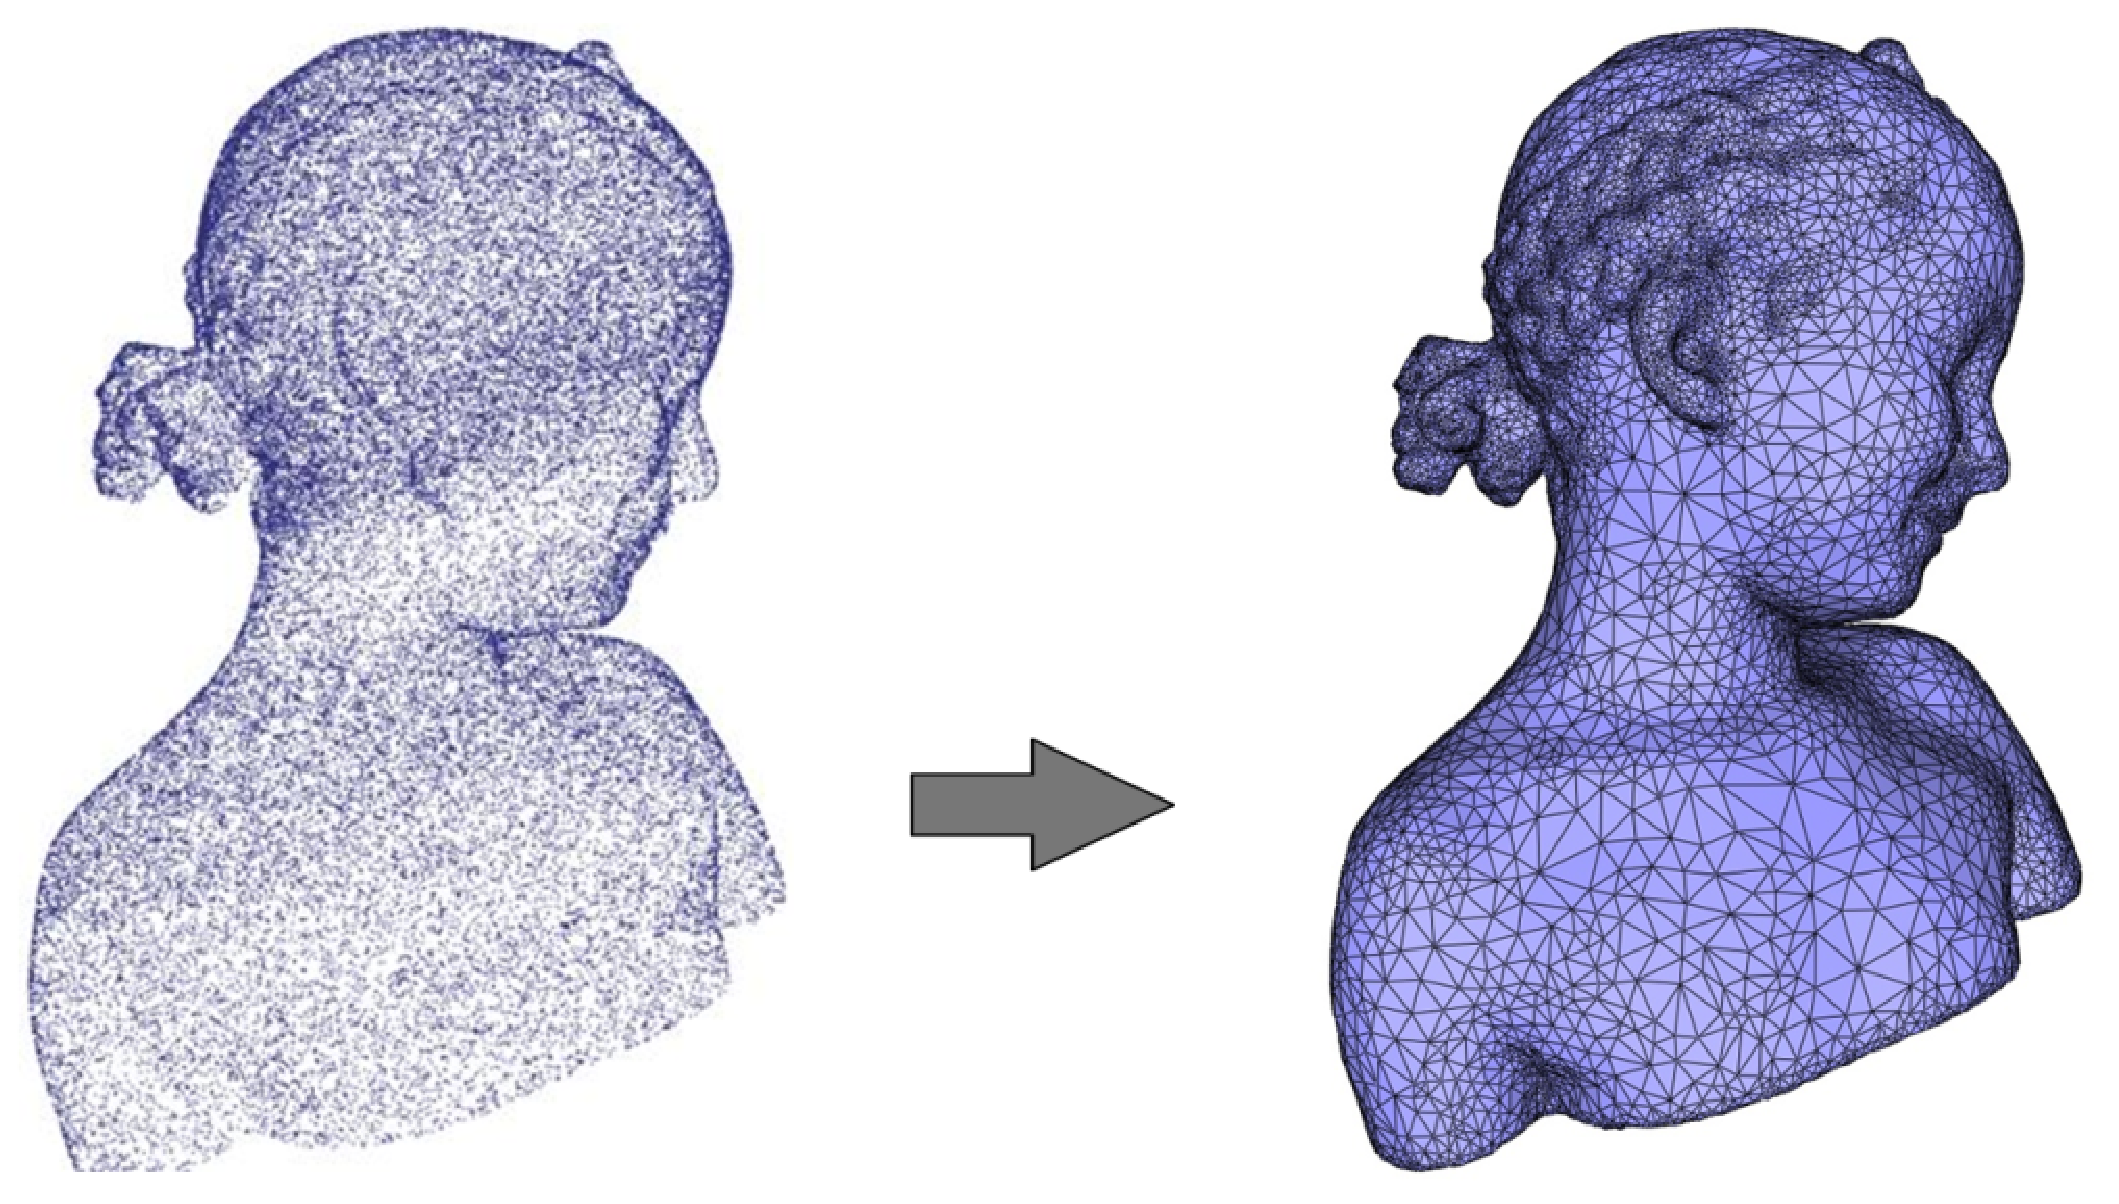
\includegraphics[width=1.0\textwidth]{Surface_reconstruction_points_3/bimba} % omit .eps suffix
    \end{ccTexOnly}
    \begin{ccHtmlOnly}
        <img width="80%" border=0 src="./bimba.png"><P>
    \end{ccHtmlOnly}
    % Title
    \begin{figure}[h]
        \caption{Poisson reconstruction.
                 Left: 120K points sampled on a statue (Minolta laser scanner).
                 Right: reconstructed surface mesh.}
    \end{figure}
\end{center}

% Insert image eros.png/.eps
\begin{center}
    \label{Surface_reconstruction_points_3-fig-eros}
    % Image
    \begin{ccTexOnly}
      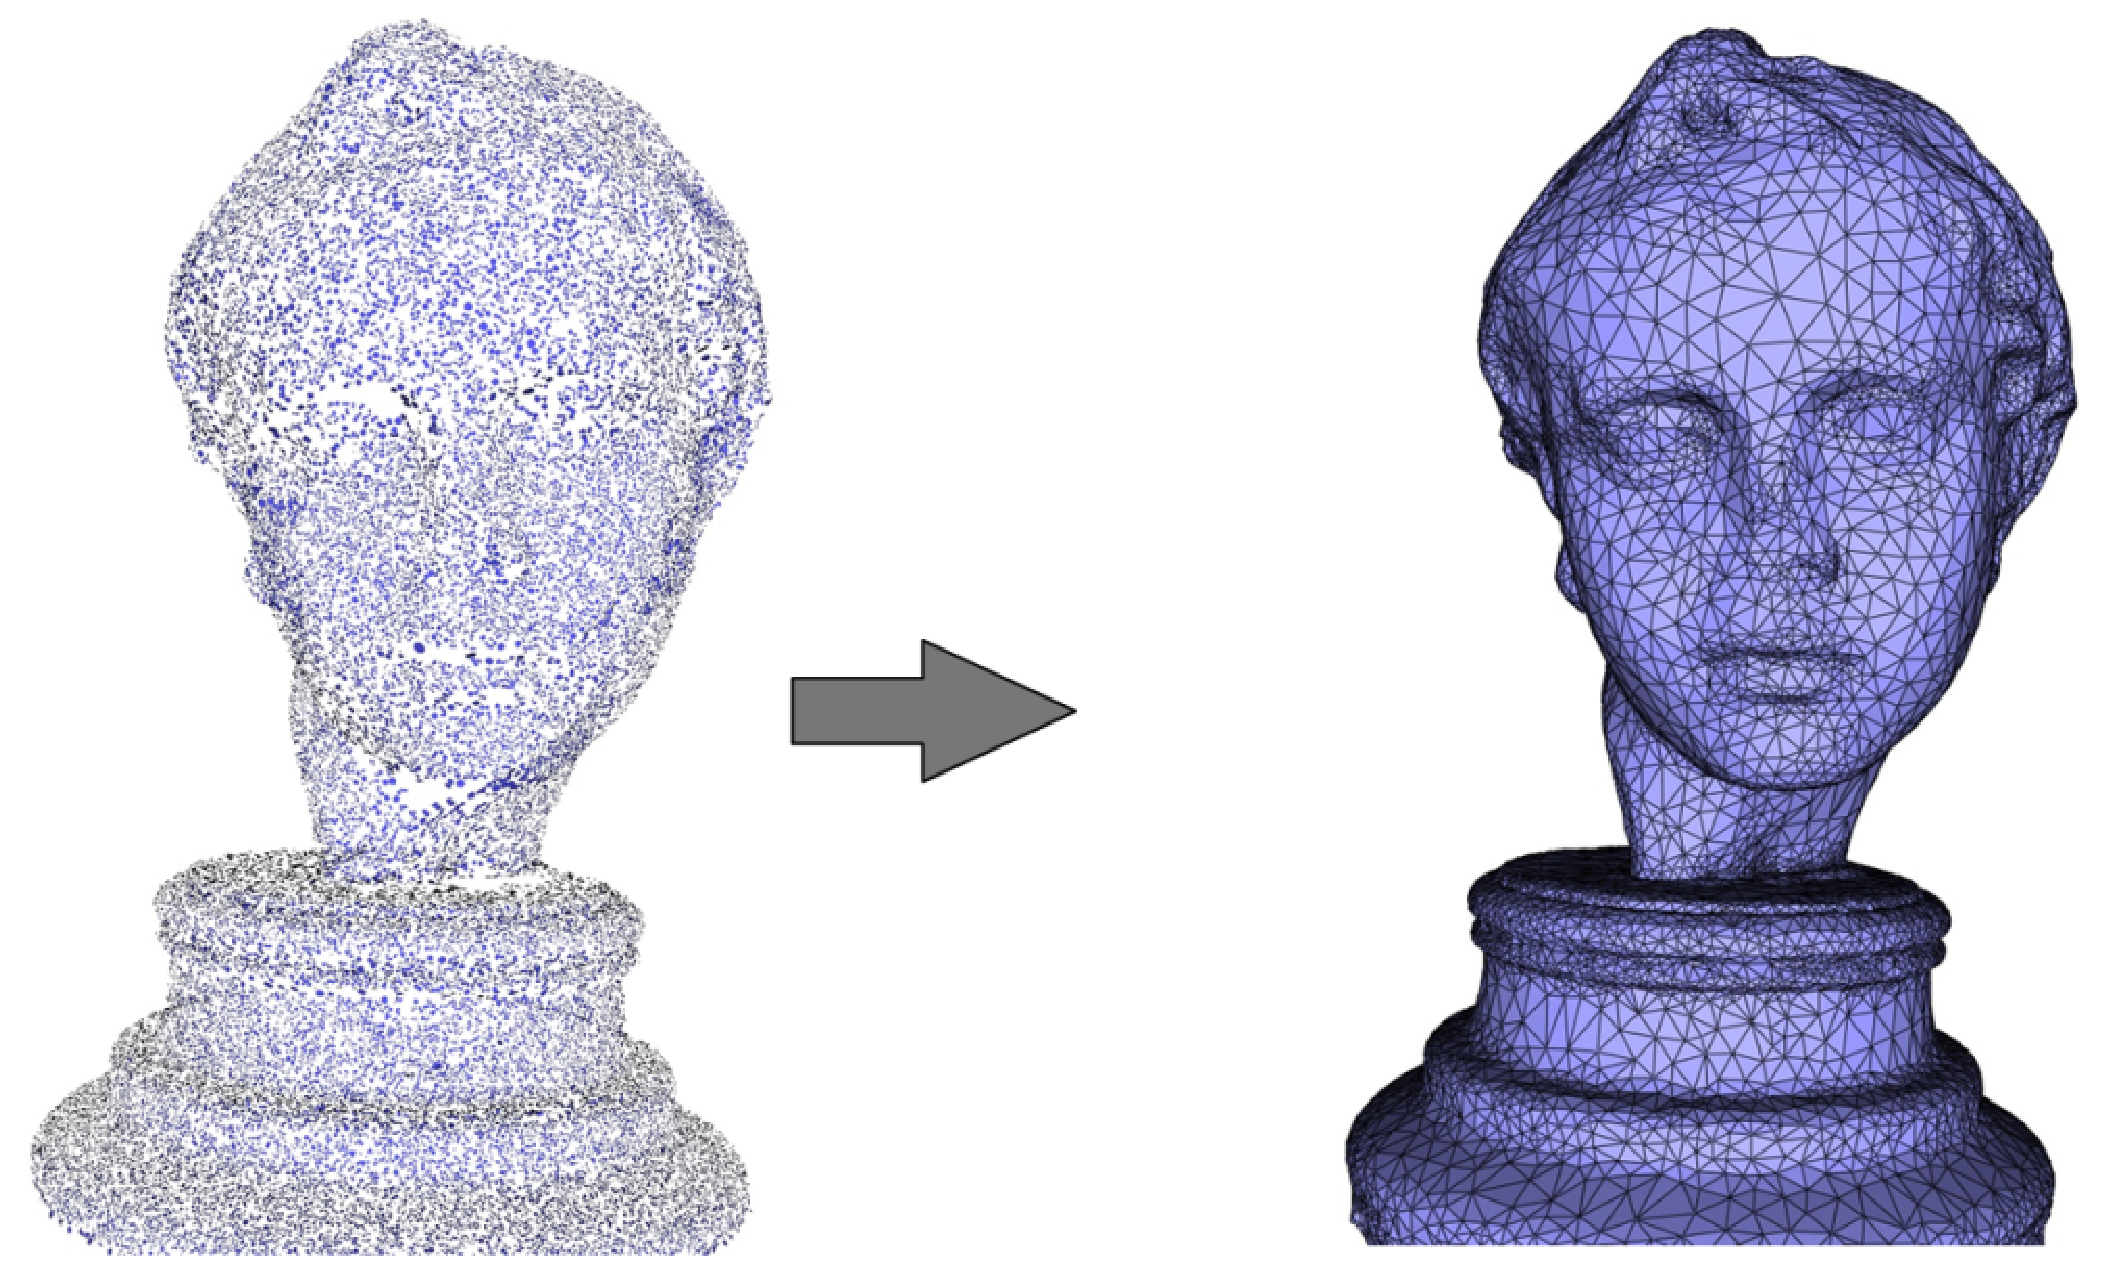
\includegraphics[width=1.0\textwidth]{Surface_reconstruction_points_3/eros} % omit .eps suffix
    \end{ccTexOnly}
    \begin{ccHtmlOnly}
        <img width="80%" border=0 src="./eros.png"><P>
    \end{ccHtmlOnly}
    % Title
    \begin{figure}[h]
        \caption{Left: 120K points sampled on a statue (Minolta laser scanner).
                 Right: reconstructed surface mesh.}
    \end{figure}
\end{center}

% Insert image holes_good.png/.eps
\begin{center}
    \label{Surface_reconstruction_points_3-fig-holes_good}
    % Image
    \begin{ccTexOnly}
      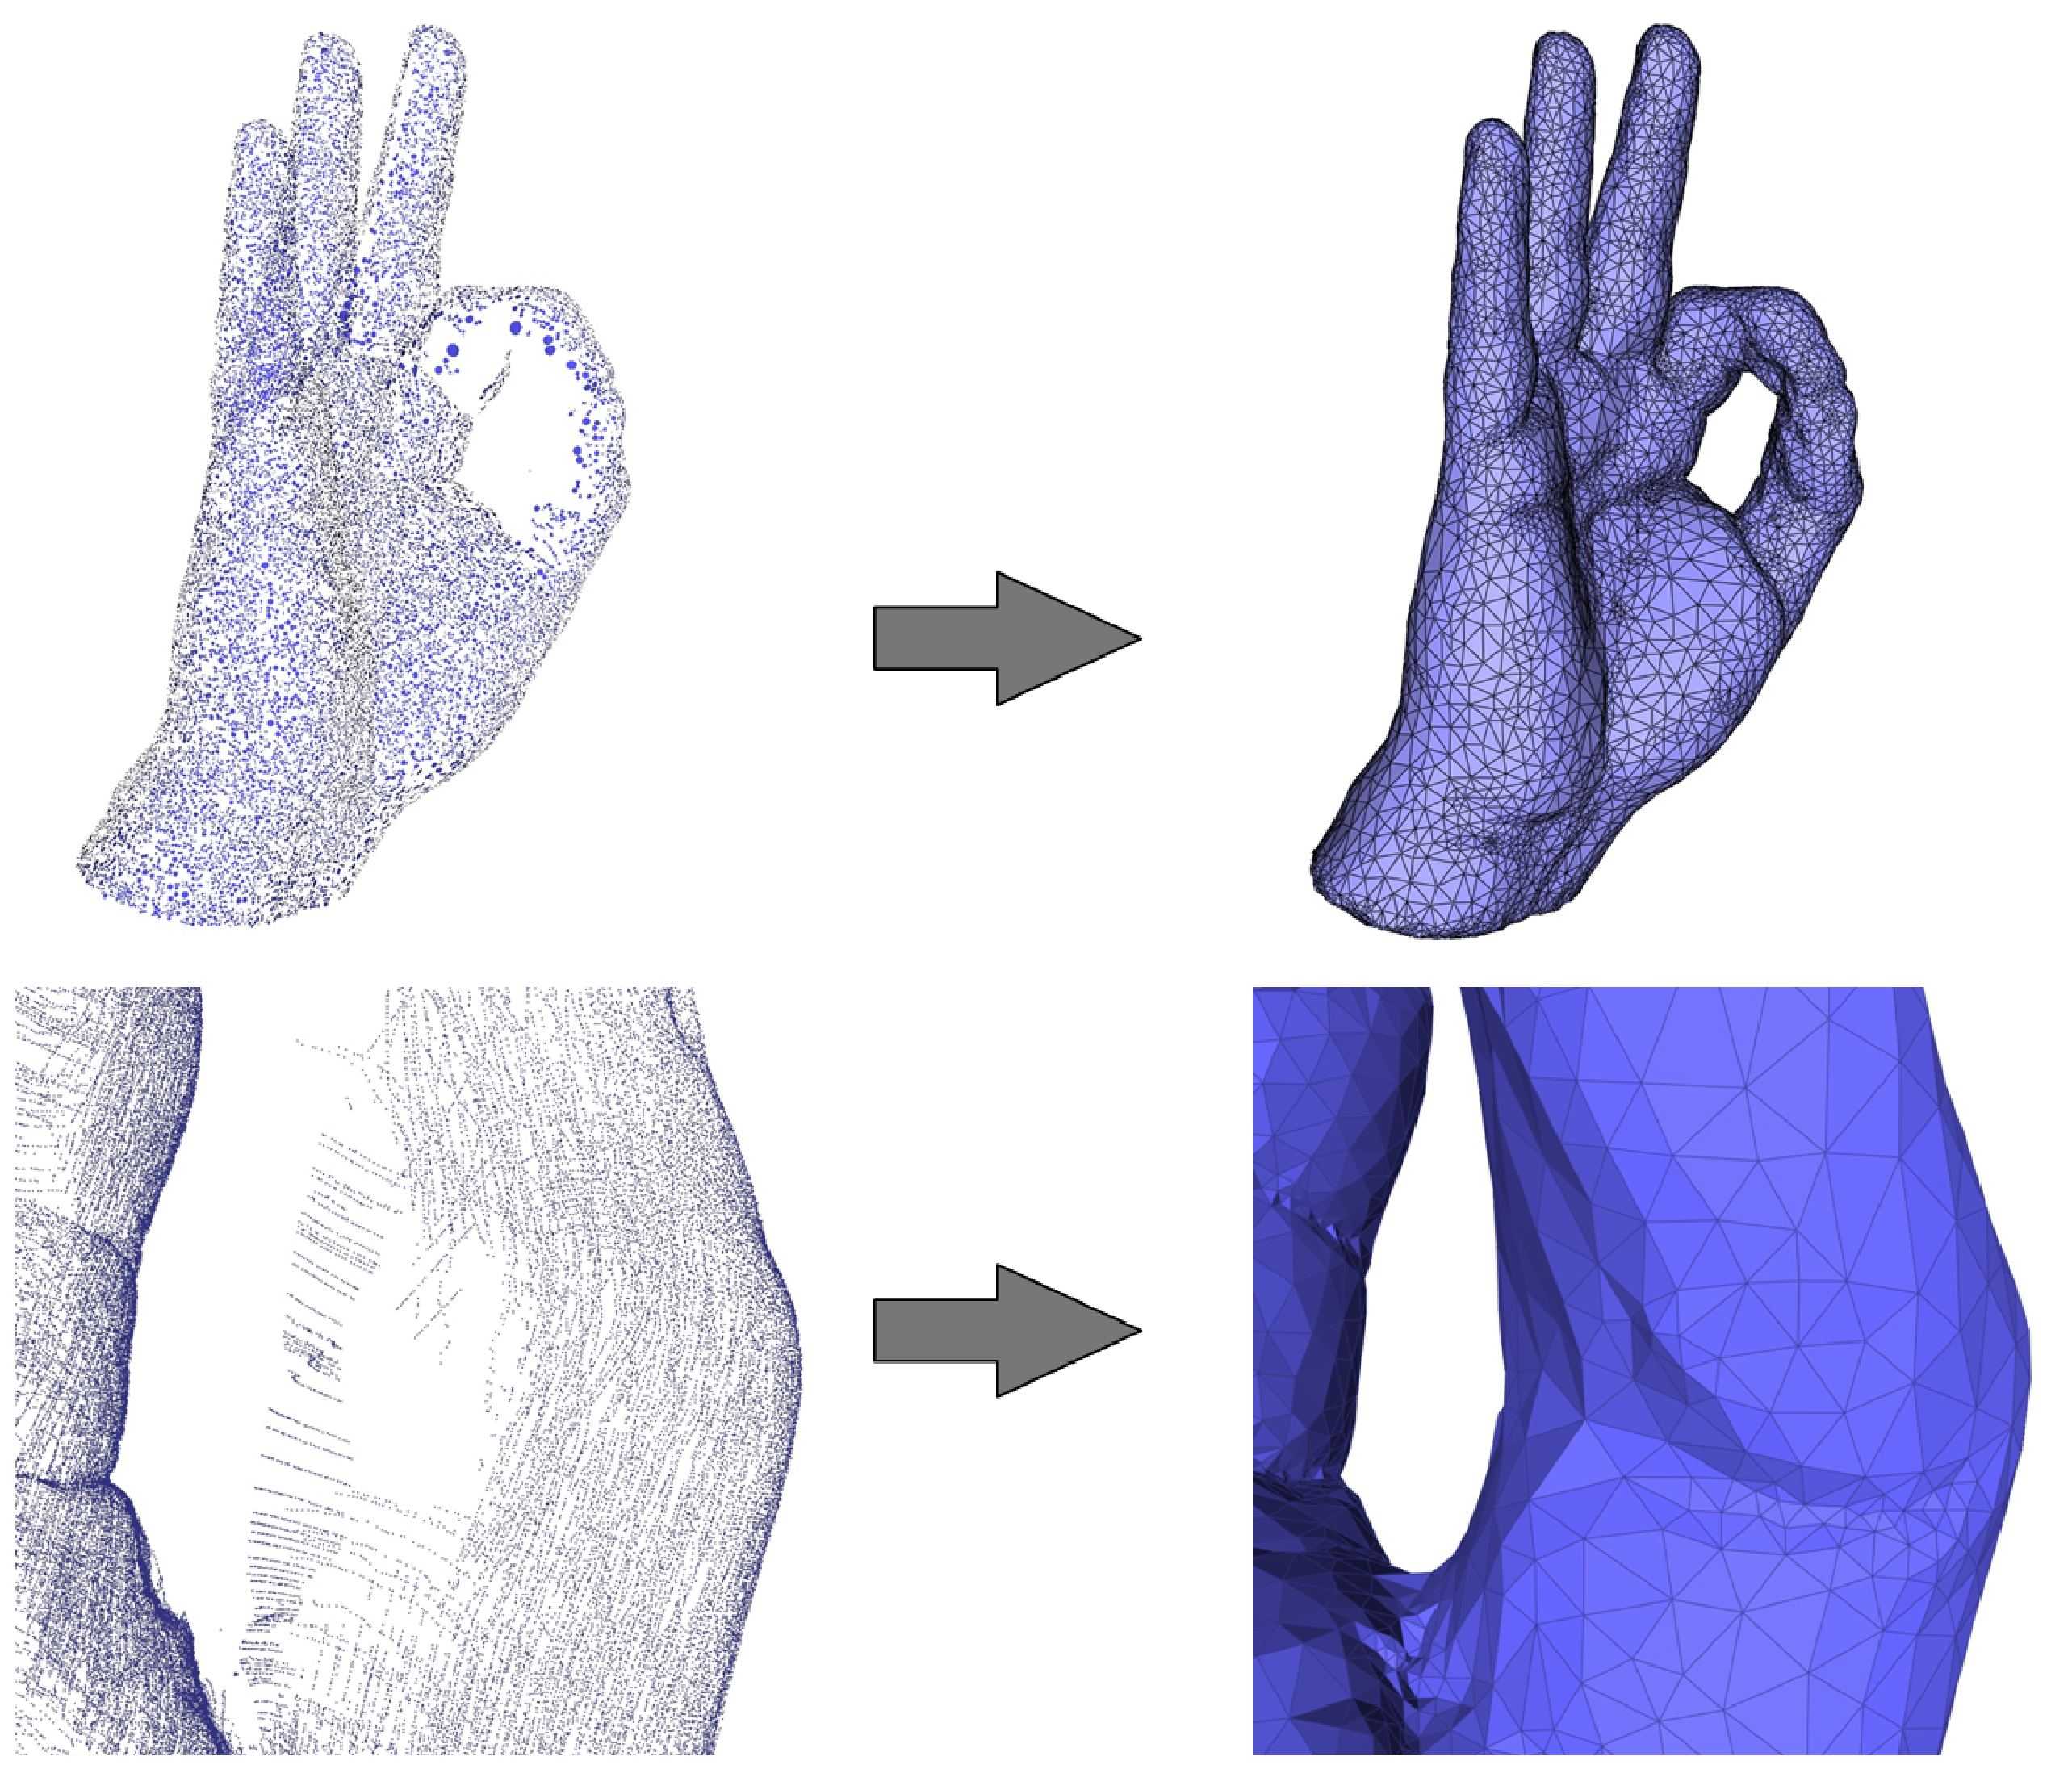
\includegraphics[width=1.0\textwidth]{Surface_reconstruction_points_3/holes_good} % omit .eps suffix
    \end{ccTexOnly}
    \begin{ccHtmlOnly}
        <img width="80%" border=0 src="./holes_good.png"><P>
    \end{ccHtmlOnly}
    % Title
    \begin{figure}[h]
        \caption{Left: 65K points sampled on hand (Kreon laser scanner).
                 Bottom-left: notice that the point set is highly anisotropic.
                 Right: reconstructed surface mesh. Notice that the hole on the fingers is properly closed.}
    \end{figure}
\end{center}

% Insert image outliers.png/.eps
\begin{center}
    \label{Surface_reconstruction_points_3-fig-outliers}
    % Image
    \begin{ccTexOnly}
      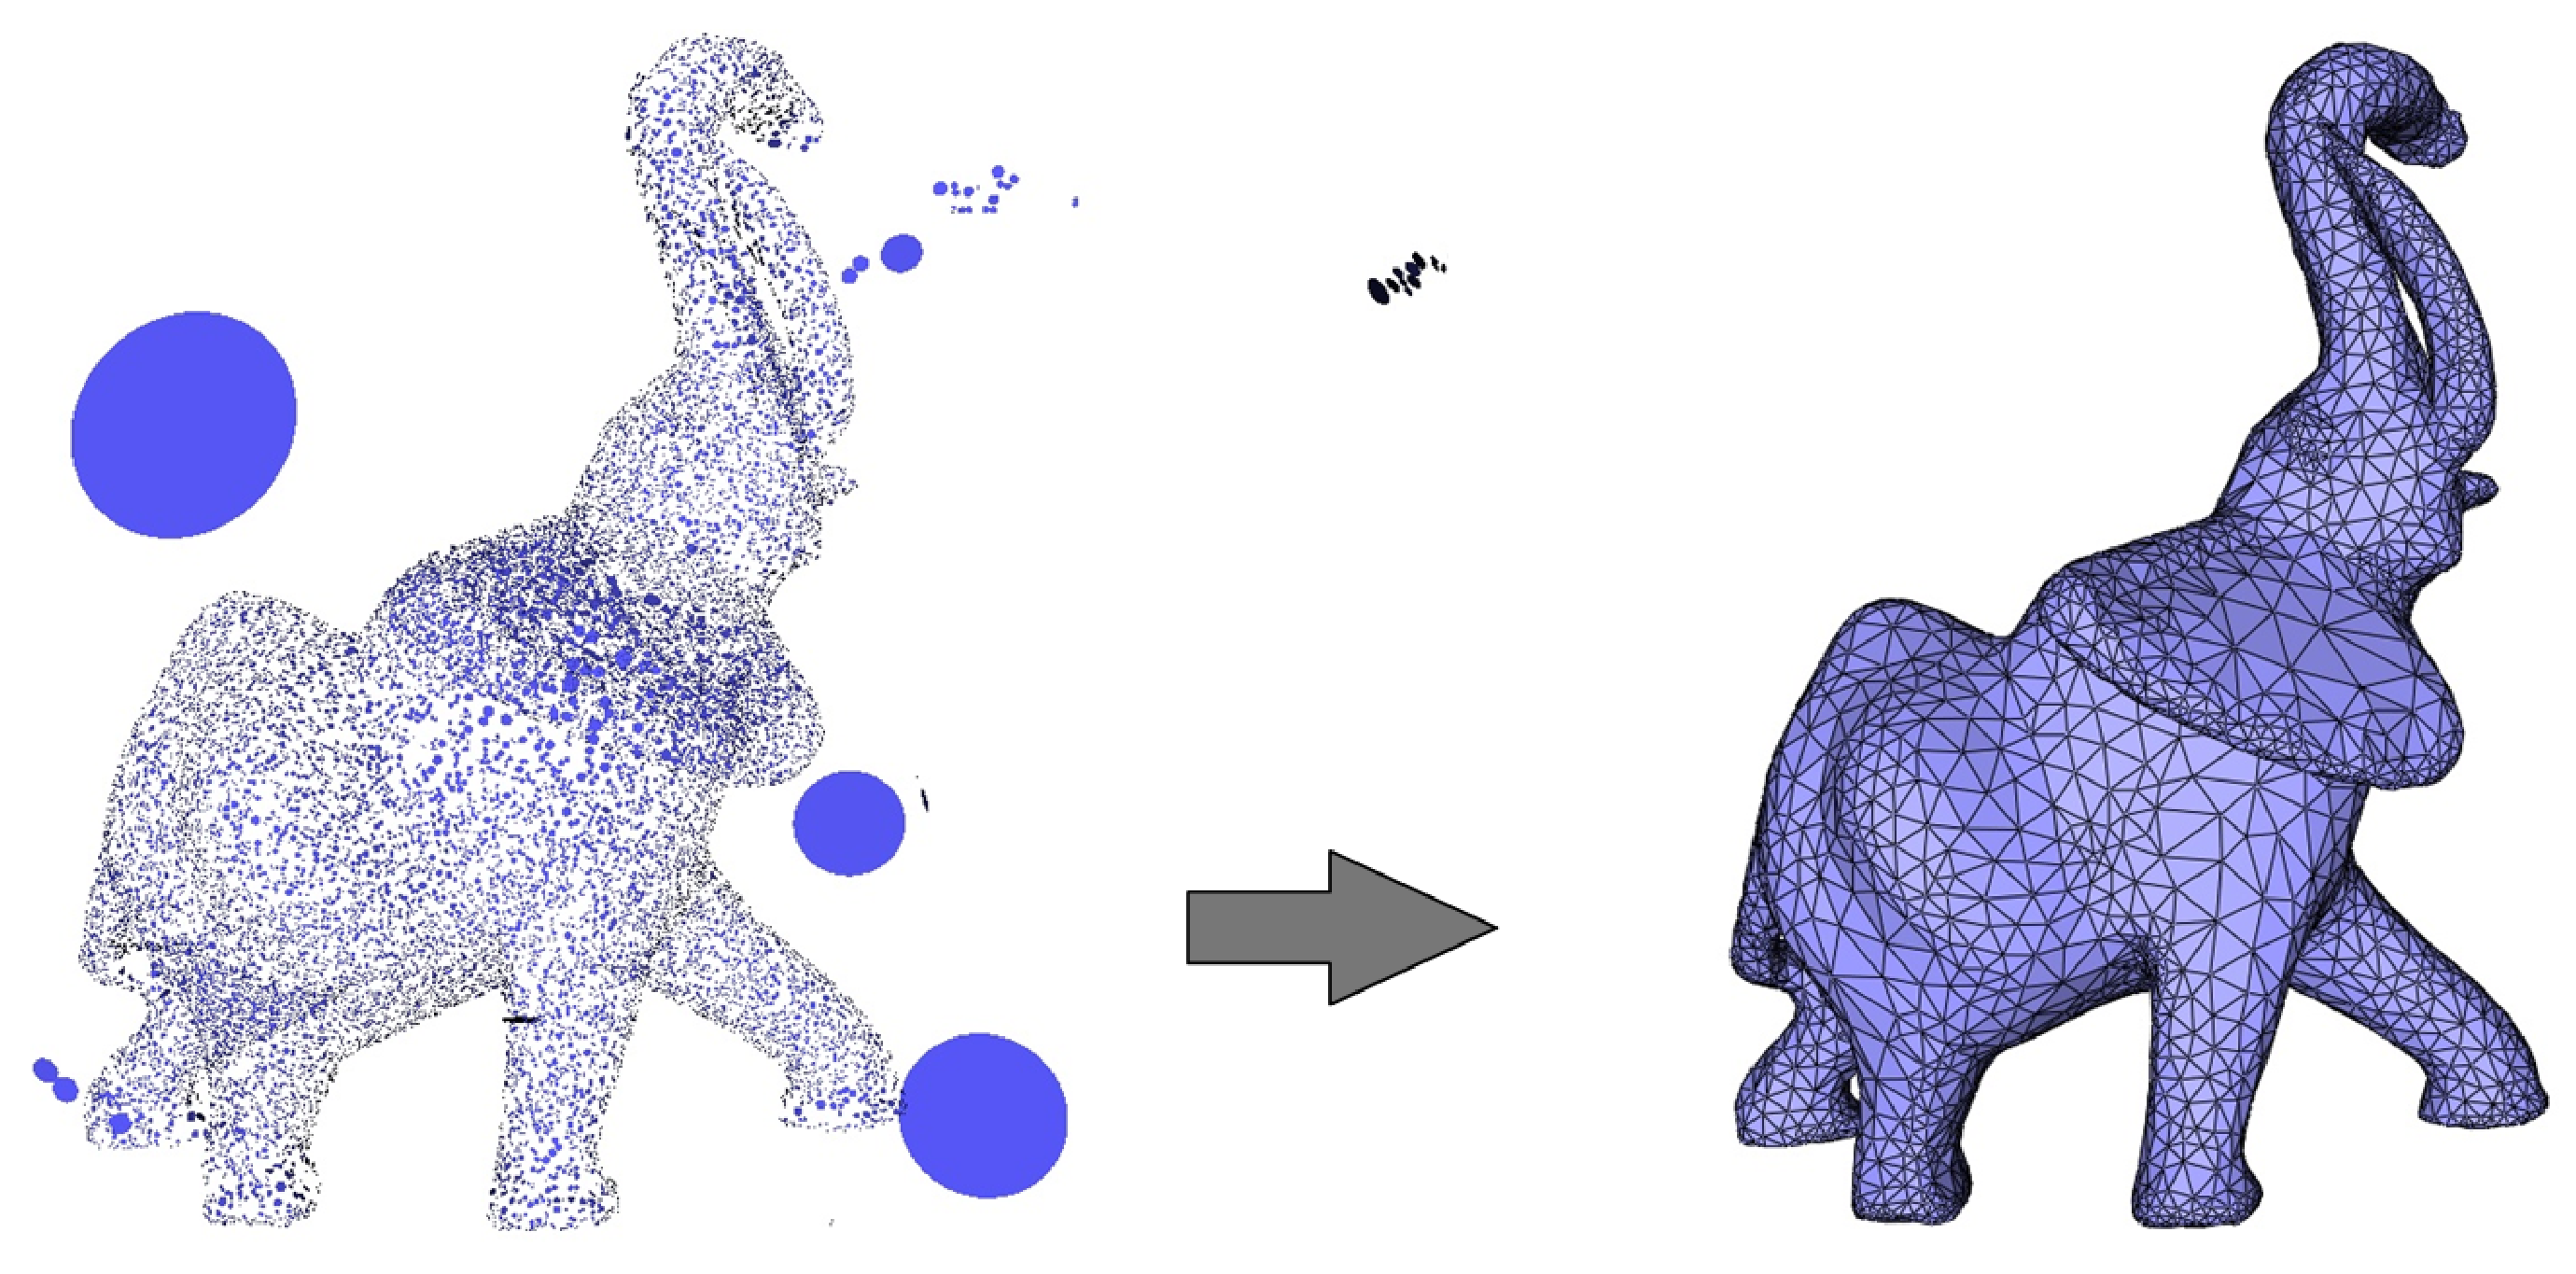
\includegraphics[width=1.0\textwidth]{Surface_reconstruction_points_3/outliers} % omit .eps suffix
    \end{ccTexOnly}
    \begin{ccHtmlOnly}
        <img width="80%" border=0 src="./outliers.png"><P>
    \end{ccHtmlOnly}
    % Title
    \begin{figure}[h]
        \caption{Left: 70K points sampled on an elephant with outliers (emphasized with circles).
                 Right: reconstructed surface mesh.}
    \end{figure}
\end{center}


\subsubsection{Contouring Parameters}

This implementation of the Poisson surface reconstruction method computes a Poisson implicit function
piecewise linear in the tetrahedra of a 3D triangulation of the input points.
On the other hand, the contouring algorithm \ccc{make_surface_mesh()} expects a smooth implicit function.
In order for the Poisson function to appear smooth, we should reconstruct meshes with edges longer than 10 input vertices.\\
\\
For this purpose, we recommend to use the next contouring parameters:
\begin{itemize}
\item Min triangle angle: 30 degrees, or less.
\item Max triangle radius: 100 * the input point set's average spacing, or more.
\item Approximation distance: 0.25 * the input point set's average spacing, or more.
\end{itemize}

% Insert image contouring_bad.png/.eps
\begin{center}
    \label{Surface_reconstruction_points_3-fig-contouring_bad}
    % Image
    \begin{ccTexOnly}
      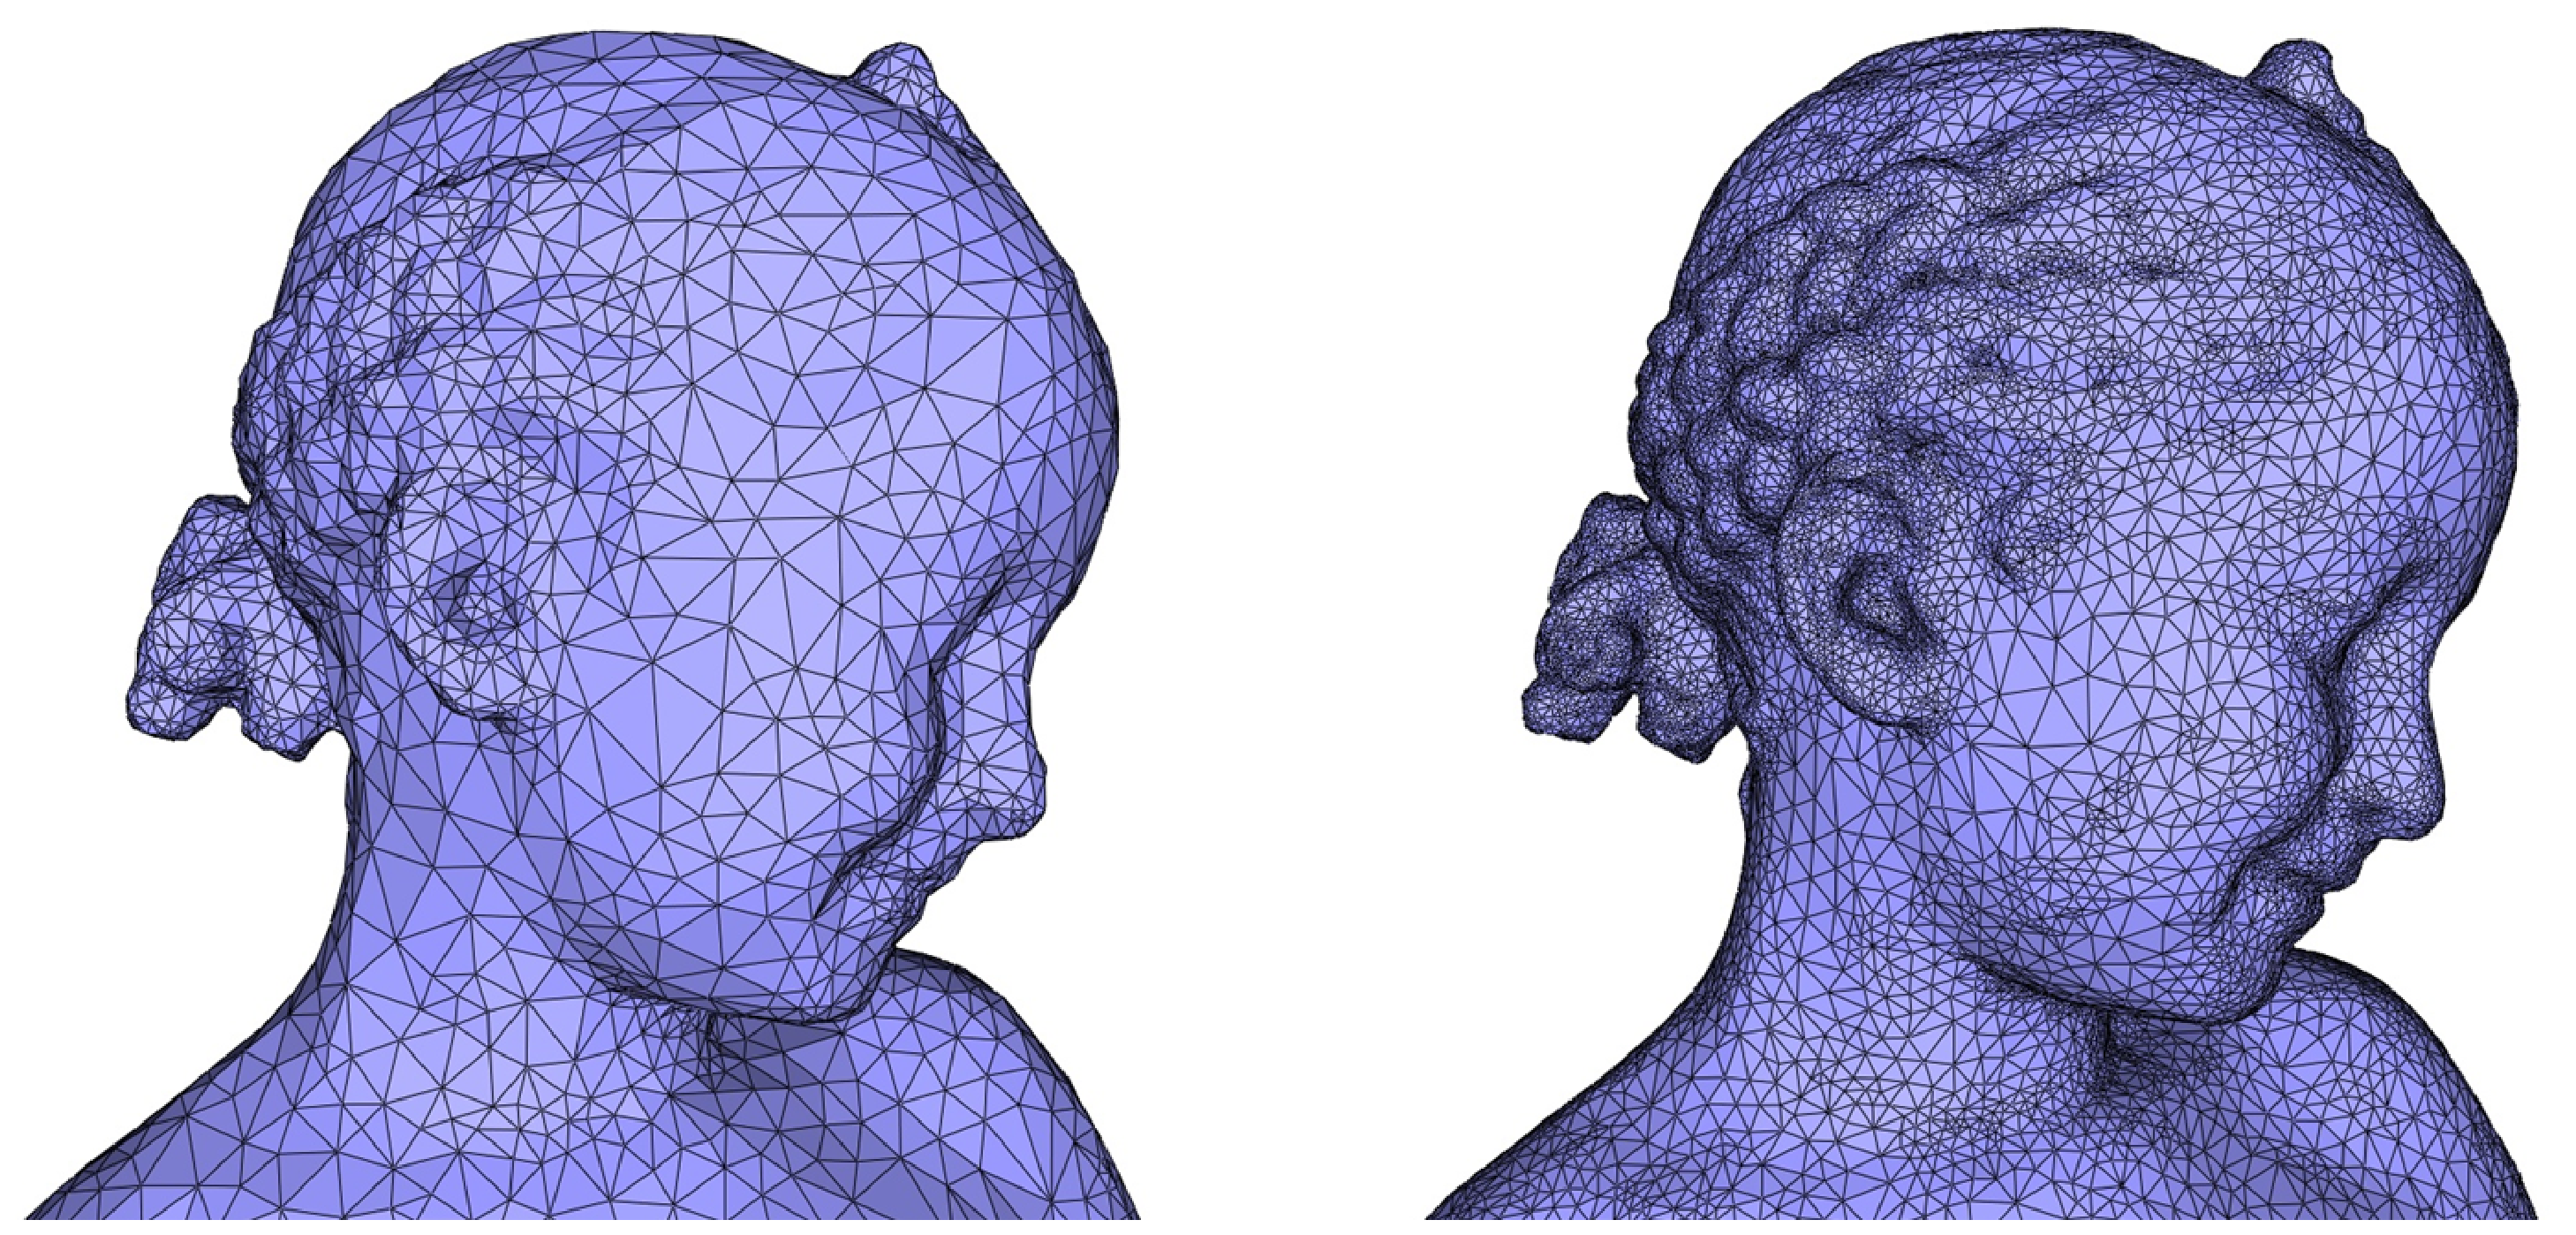
\includegraphics[width=1.0\textwidth]{Surface_reconstruction_points_3/contouring_bad} % omit .eps suffix
    \end{ccTexOnly}
    \begin{ccHtmlOnly}
        <img width="80%" border=0 src="./contouring_bad.png"><P>
    \end{ccHtmlOnly}
    % Title
    \begin{figure}[h]
        \caption{Left: surface reconstructed with approximation distance = 0.25 * average spacing.
                 Right: surface reconstructed with approximation distance = 0.15 * average spacing.
                 Notice the small triangles on the girl's chick at the frontier between two underlying tetrahedra.}
    \end{figure}
\end{center}




\subsection{Degraded Conditions}

\subsubsection{Holes}

By construction, this method contours the zero level set of an implicit function and reconstructs a closed mesh.\\
For small holes, this is probably what you expect. \\
In case of large holes that you do not want to close or that you want to close with a plane, you will need a postprocessing stage.

% Insert image holes_bad.png/.eps
\begin{center}
    \label{Surface_reconstruction_points_3-fig-holes_bad}
    % Image
    \begin{ccTexOnly}
      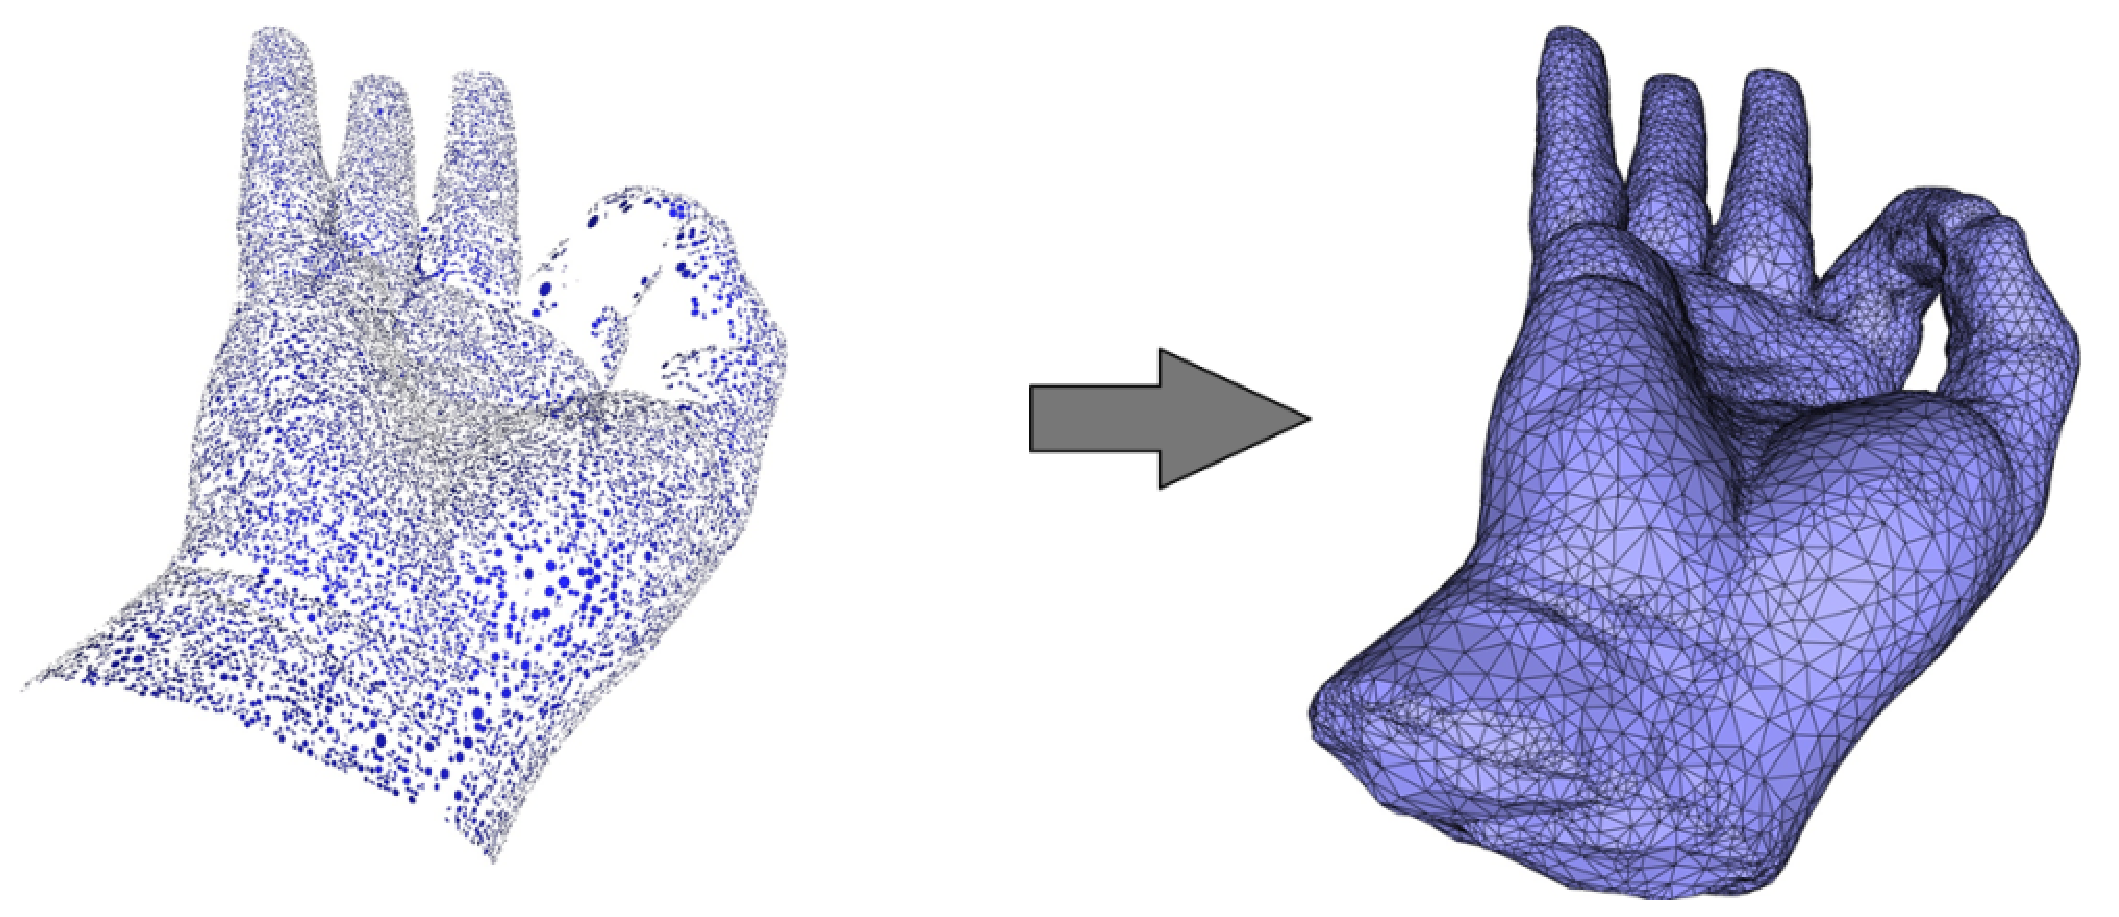
\includegraphics[width=0.5\textwidth]{Surface_reconstruction_points_3/holes_bad} % omit .eps suffix
    \end{ccTexOnly}
    \begin{ccHtmlOnly}
        <img width="50%" border=0 src="./holes_bad.png"><P>
    \end{ccHtmlOnly}
    % Title
    \begin{figure}[h]
        \caption{Left: 65K points sampled on hand with no data captured at the wrist base.
                 Right: reconstructed surface mesh. Notice that surface is properly closed on the fingers
                 but also closed at the wrist in a non-natural way.}
    \end{figure}
\end{center}


\subsubsection{Noise}

Poisson reconstruction method supports noise if the approximation distance requested at the contouring stage is large w.r.t. the noise.\\
If you wish to use a small approximation distance, you may remove noise as a preprocessing step using \ccc{CGAL::jet_smooth_point_set()}.

% Insert image noise.png/.eps
\begin{center}
    \label{Surface_reconstruction_points_3-fig-noise}
    % Image
    \begin{ccTexOnly}
      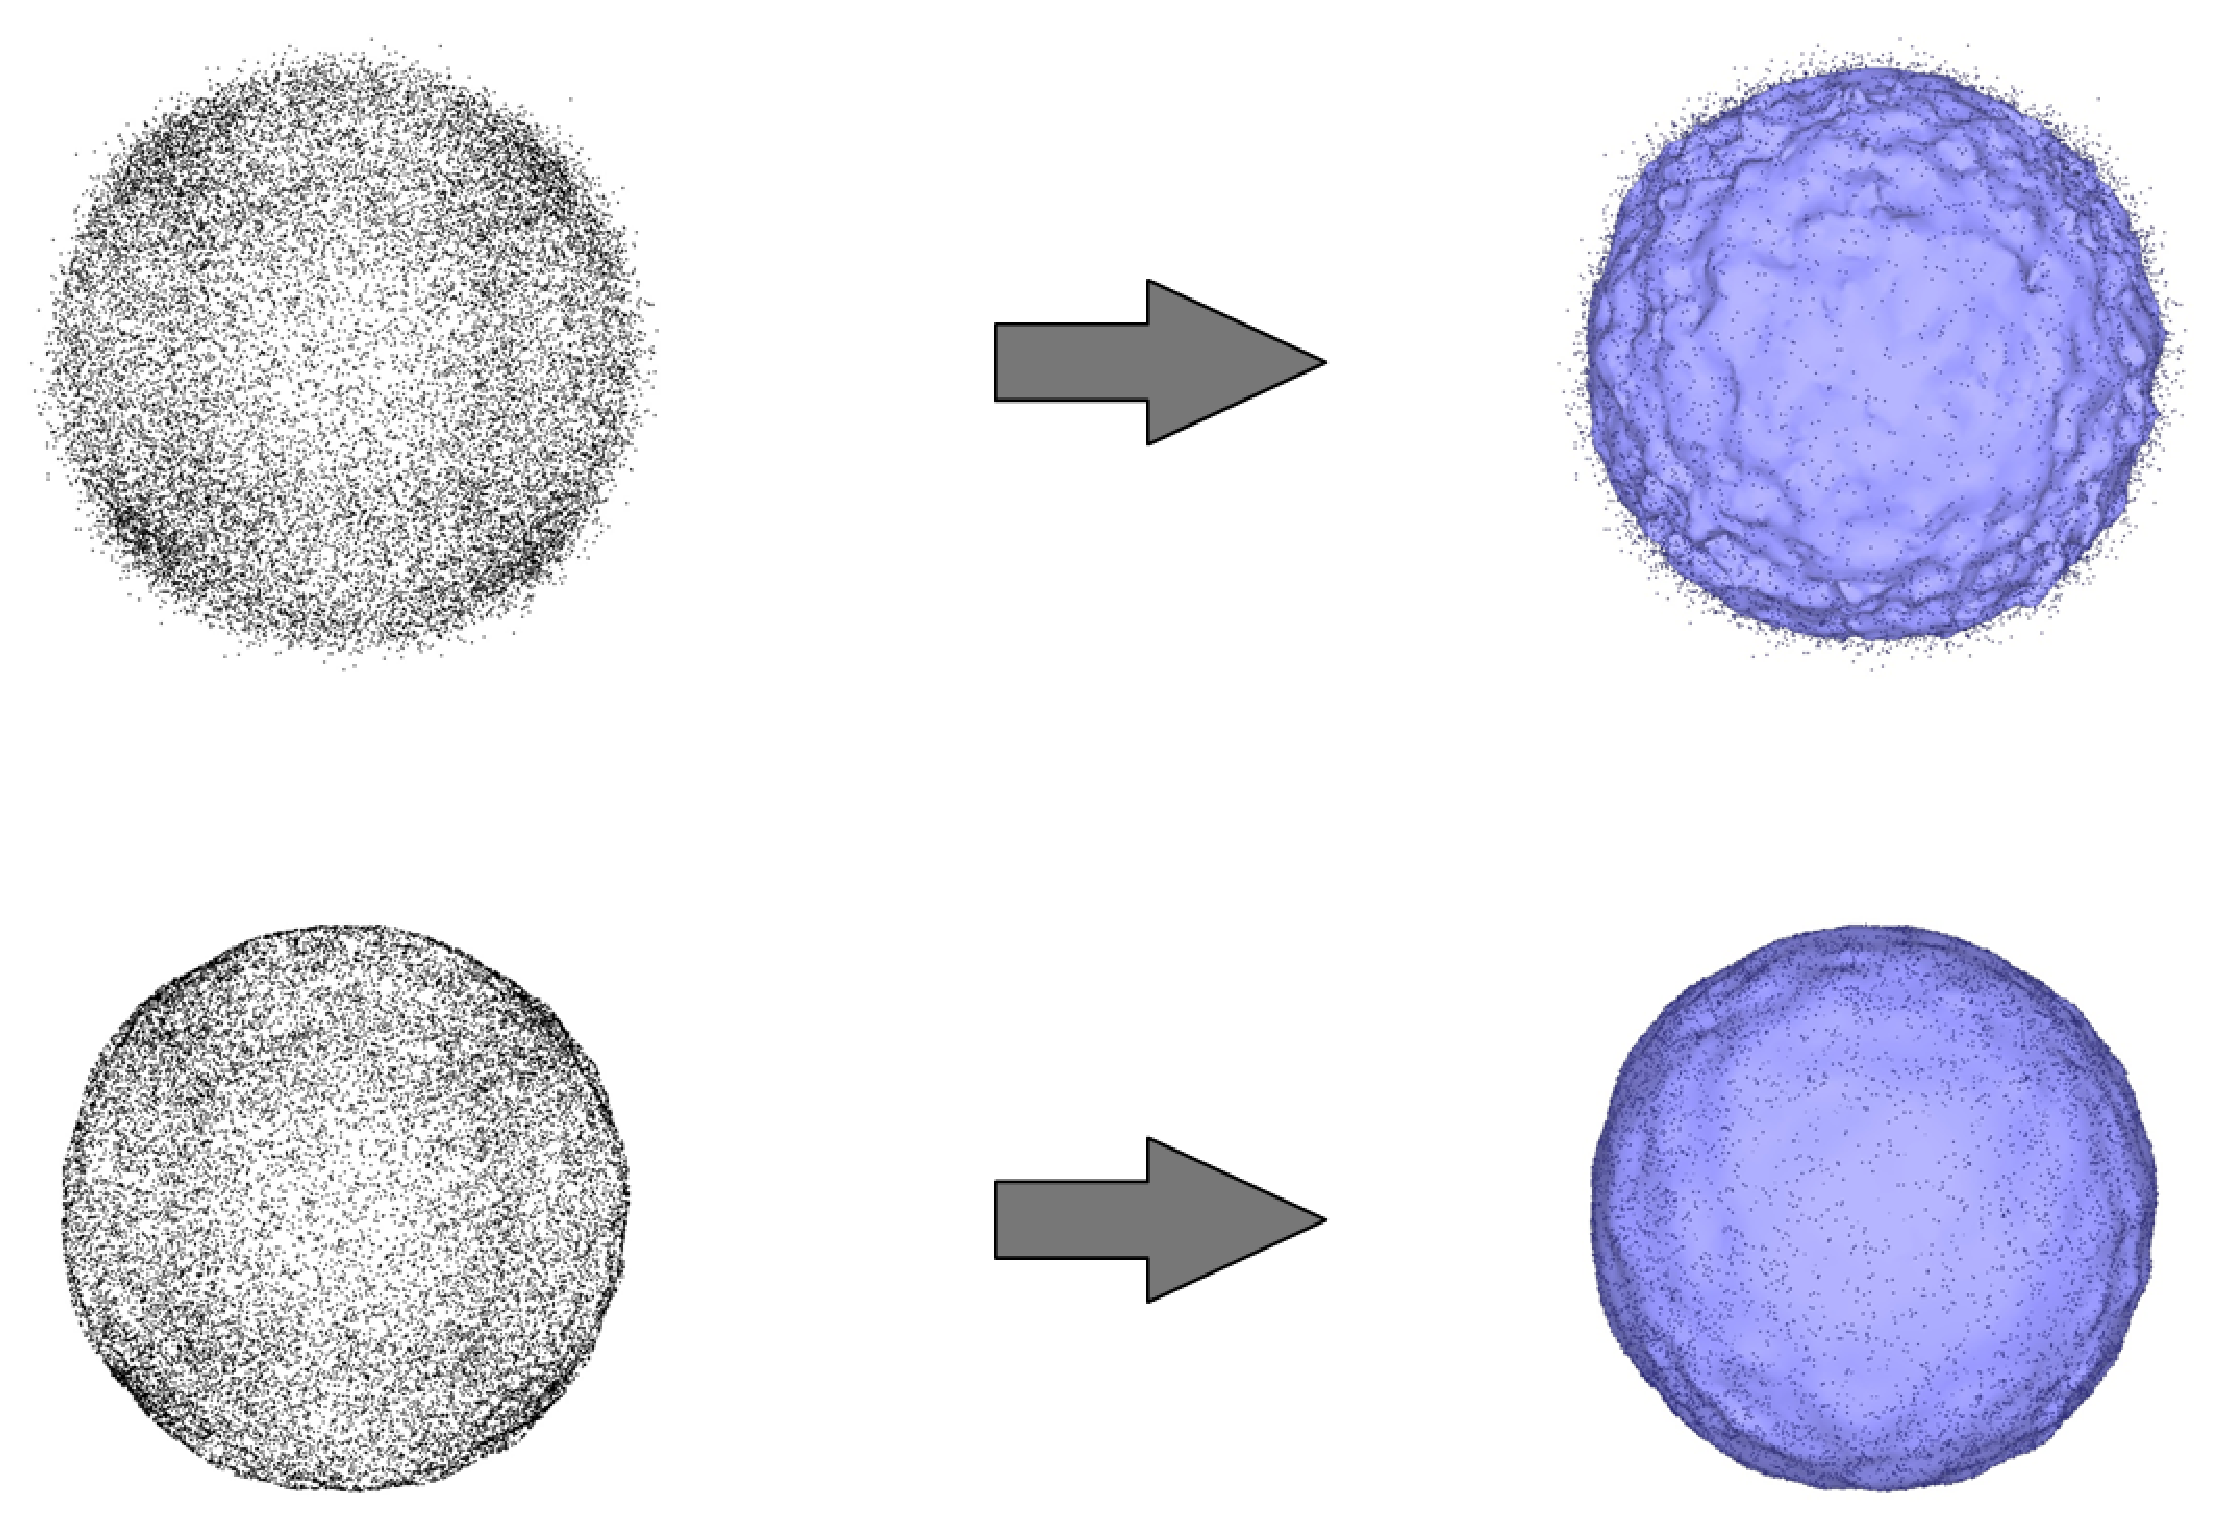
\includegraphics[width=0.5\textwidth]{Surface_reconstruction_points_3/noise} % omit .eps suffix
    \end{ccTexOnly}
    \begin{ccHtmlOnly}
        <img width="50%" border=0 src="./noise.png"><P>
    \end{ccHtmlOnly}
    % Title
    \begin{figure}[h]
        \caption{Top-left: points sampled on sphere with a lot of noise.
                 Top-right: reconstructed surface mesh. Notice the bumps.
                 Bottom-left: smoothed point set.
                 Bottom-right: reconstructed surface mesh.}
    \end{figure}
\end{center}


\subsubsection{Outliers}

Poisson reconstruction method supports a small amount of outliers (see elephant example above).\\
Large clusters of outliers should be removed as a preprocessing step using \ccc{CGAL::remove_outliers()}.


\subsubsection{Sampling}

Poisson surface reconstruction method expects a dense point set, respecting the epsilon-sampling condition:
the input points spacing must be 10 times smaller than the local feature size. When this condition is not respected, the reconstruction may miss thin undersampled regions.

% Insert image sampling.png/.eps
\begin{center}
    \label{Surface_reconstruction_points_3-fig-sampling}
    % Image
    \begin{ccTexOnly}
      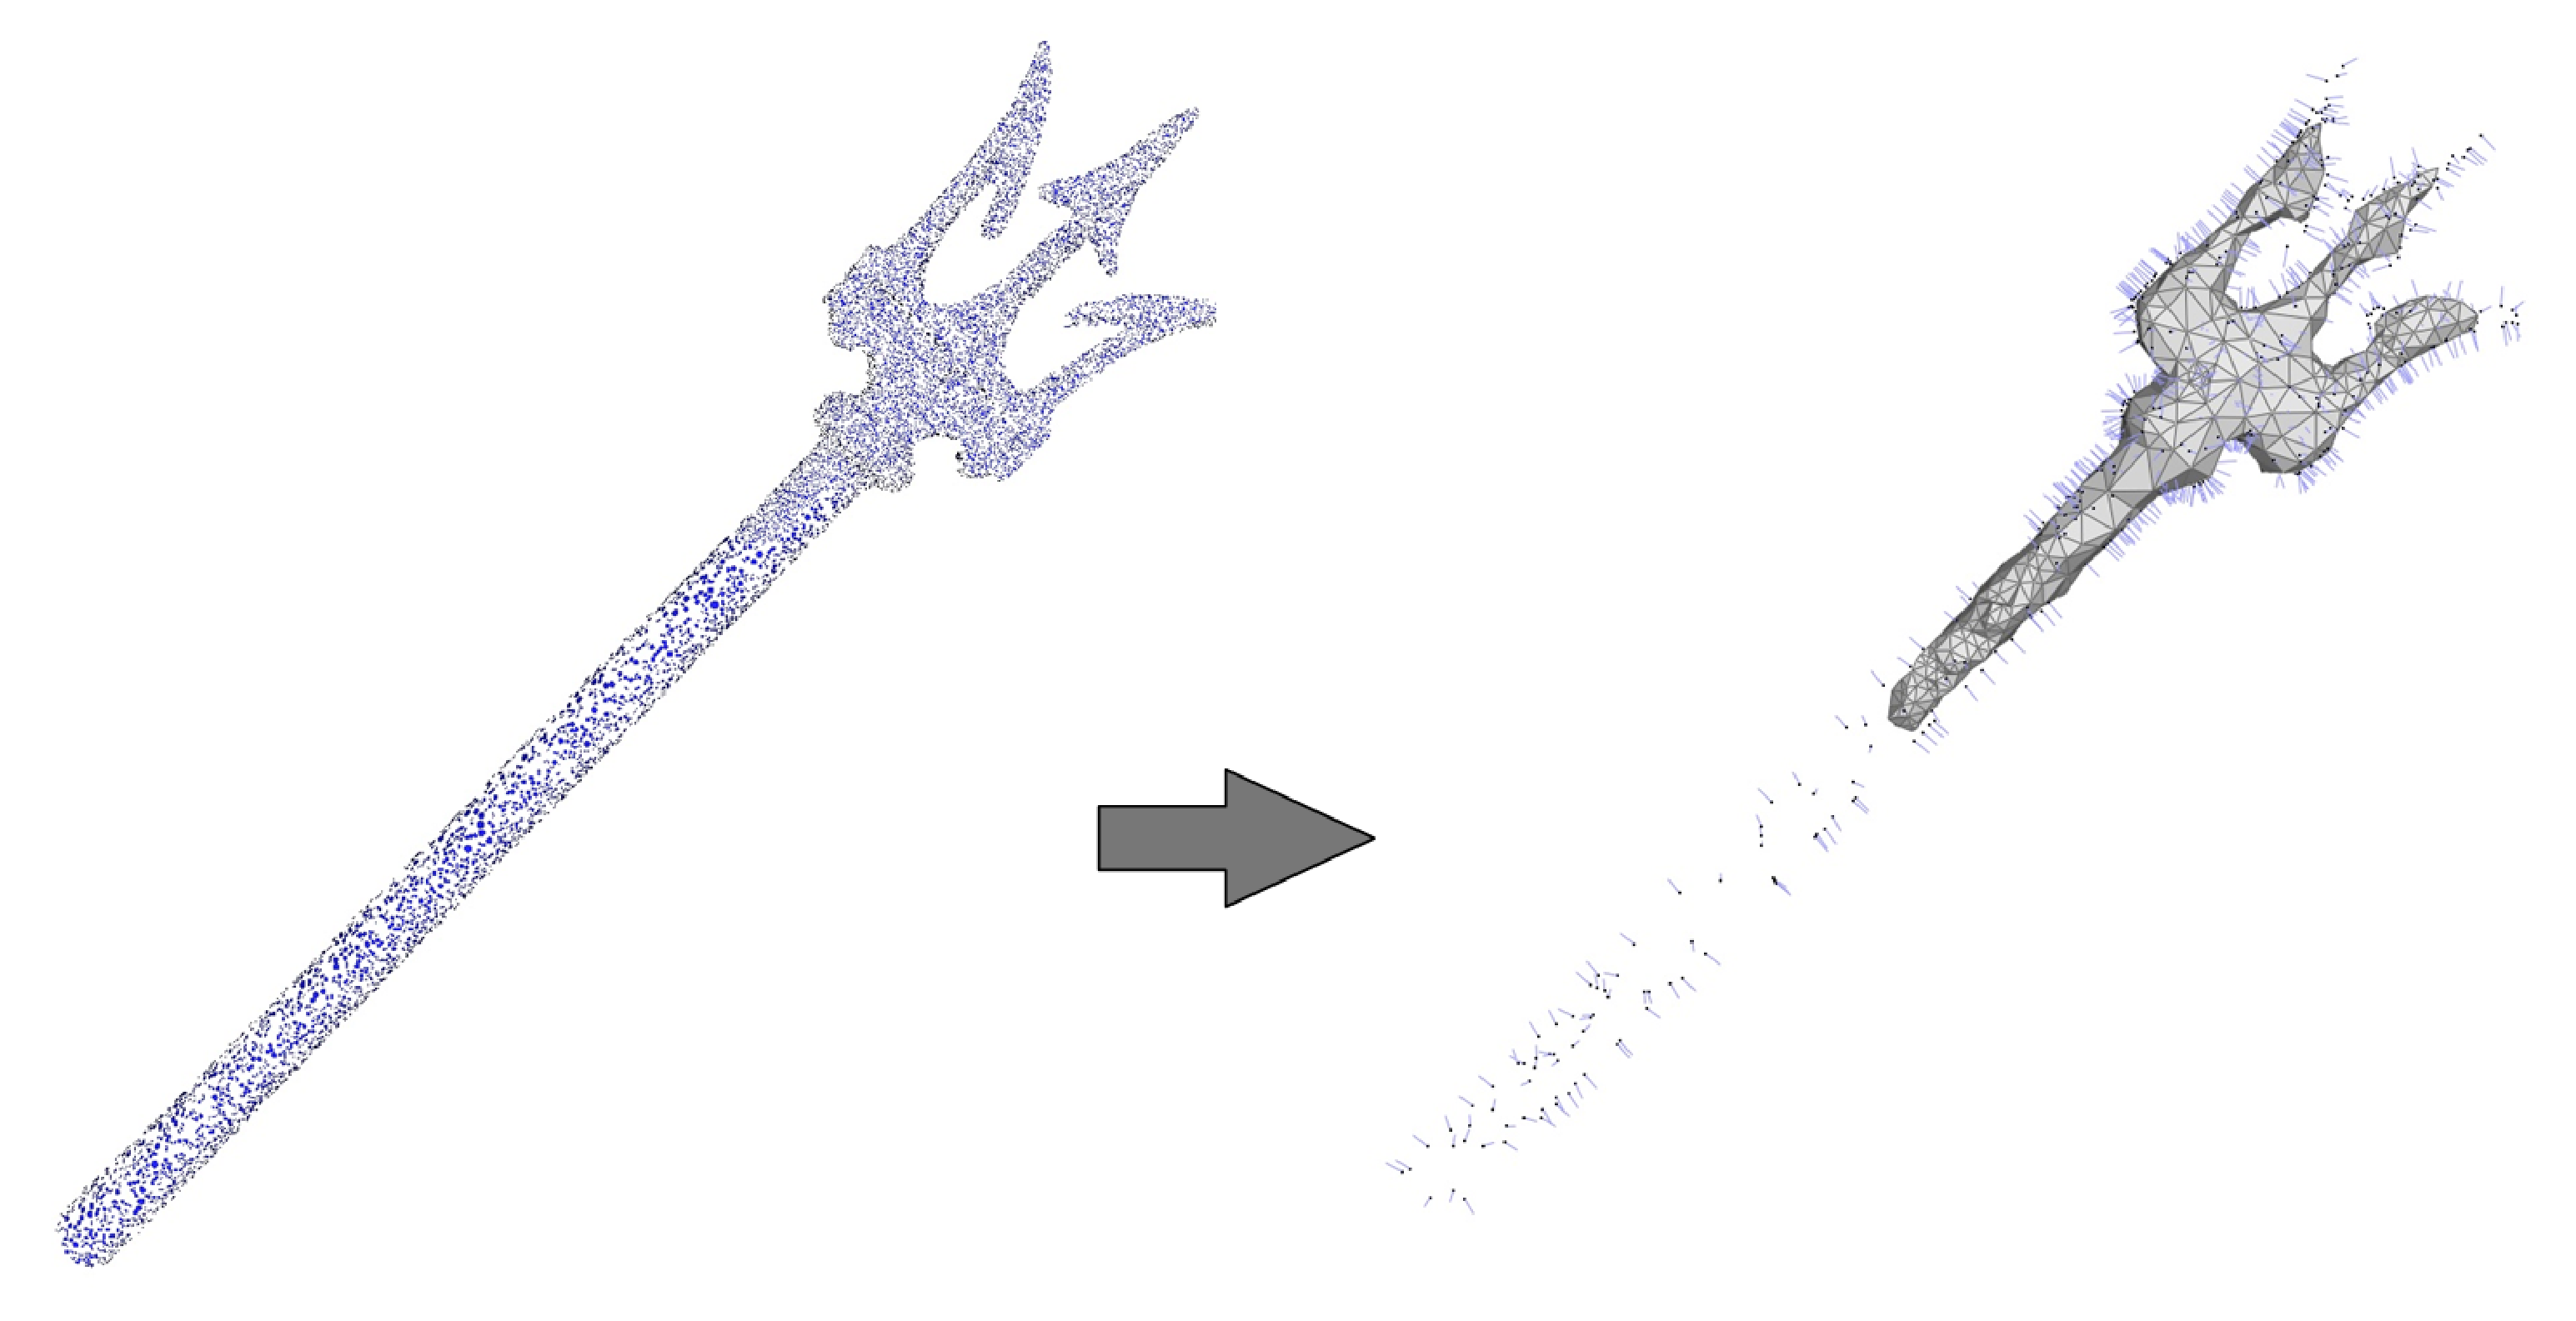
\includegraphics[width=0.5\textwidth]{Surface_reconstruction_points_3/sampling} % omit .eps suffix
    \end{ccTexOnly}
    \begin{ccHtmlOnly}
        <img width="50%" border=0 src="./sampling.png"><P>
    \end{ccHtmlOnly}
    % Title
    \begin{figure}[h]
        \caption{Left: 50K points sampled on a Neptune trident.
                 Right: point set simplified to 1K and then reconstructed
                 (input points are drawn with normals to show the missed region).}
    \end{figure}
\end{center}


\subsubsection{Normals}

As Poisson surface reconstruction solves a global linear system in the least square sense, it supports isolated flipped normals.
On the other hand, a cluster of wrong normals will lead to an incorrect implicit function.

% Insert image flipped_normals.png/.eps
\begin{center}
    \label{Surface_reconstruction_points_3-fig-flipped_normals}
    % Image
    \begin{ccTexOnly}
      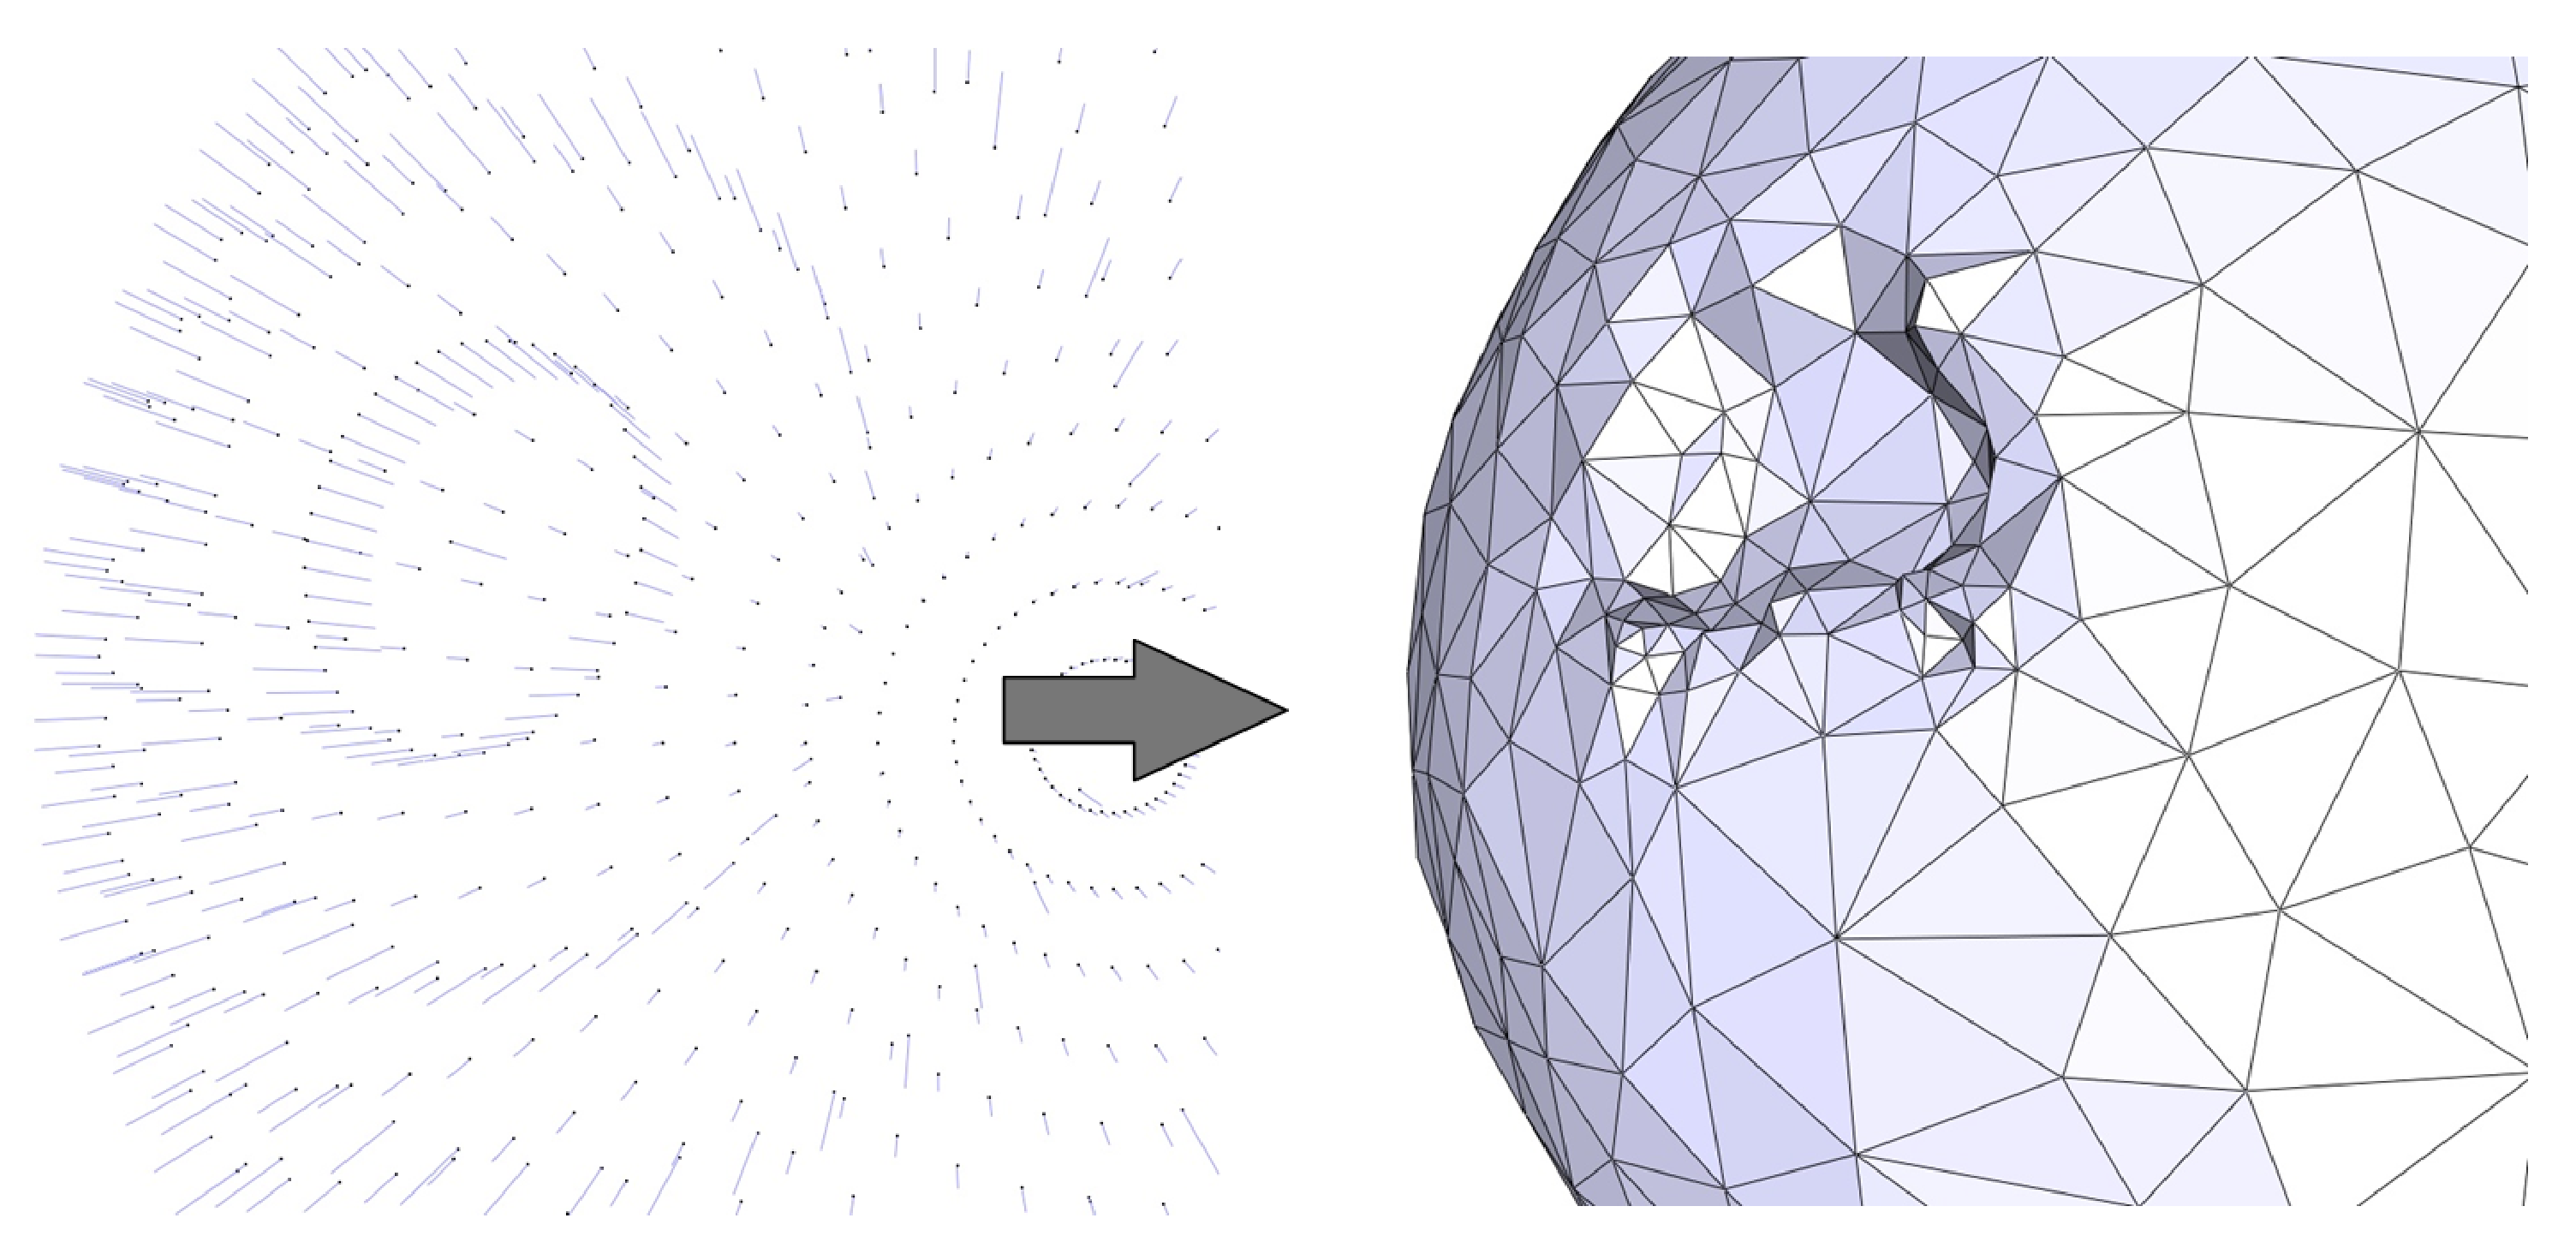
\includegraphics[width=0.5\textwidth]{Surface_reconstruction_points_3/flipped_normals} % omit .eps suffix
    \end{ccTexOnly}
    \begin{ccHtmlOnly}
        <img width="50%" border=0 src="./flipped_normals.png"><P>
    \end{ccHtmlOnly}
    % Title
    \begin{figure}[h]
        \caption{Left: points sampled on a sphere with a cluster of flipped normals.
                 Right: reconstructed surface mesh. Notice the bump in the surface.}
    \end{figure}
\end{center}


\subsubsection{Sharp Features}

Poisson surface reconstruction does not support sharp features.

% Insert image sharp_features.png/.eps
\begin{center}
    \label{Surface_reconstruction_points_3-fig-sharp_features}
    % Image
    \begin{ccTexOnly}
      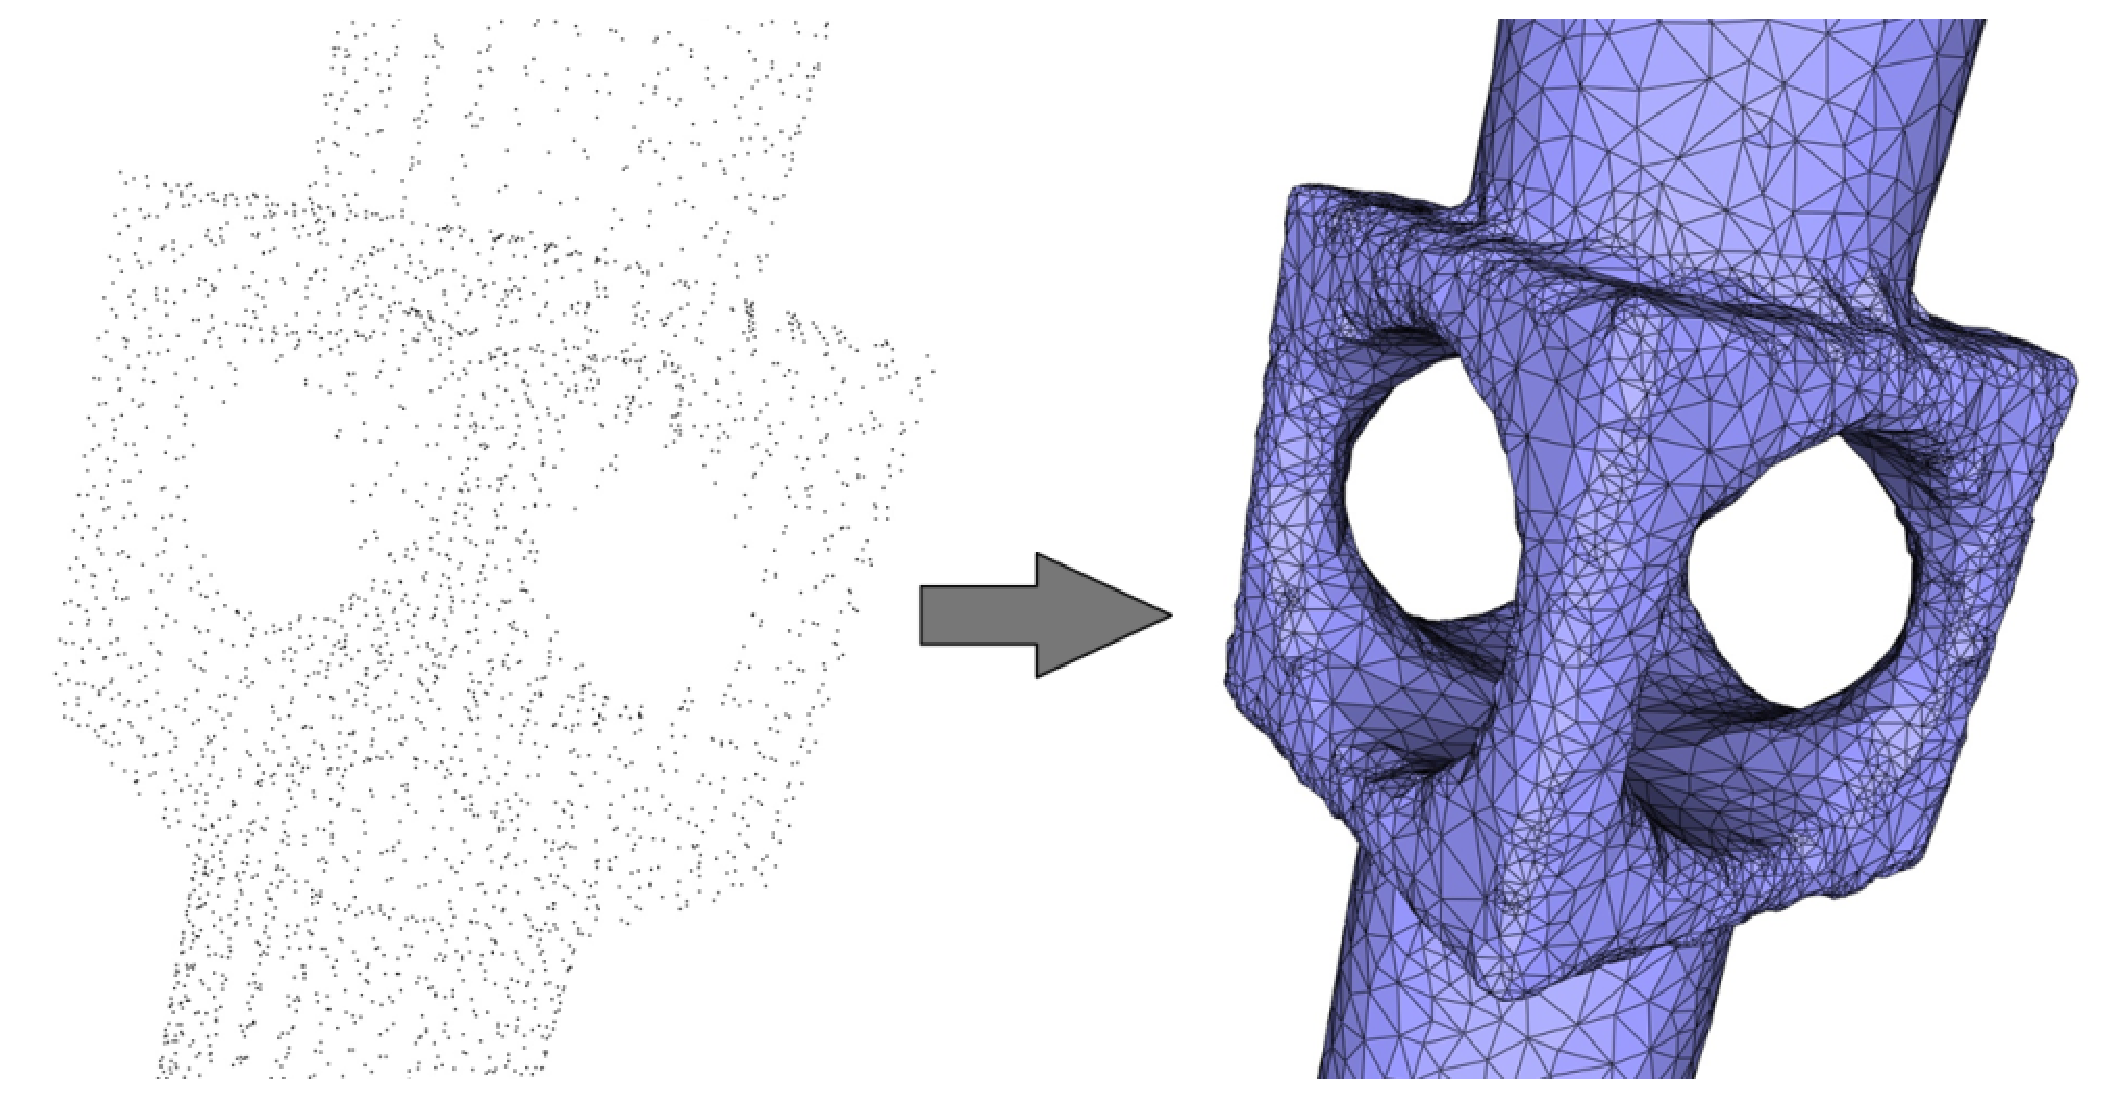
\includegraphics[width=0.5\textwidth]{Surface_reconstruction_points_3/sharp_features} % omit .eps suffix
    \end{ccTexOnly}
    \begin{ccHtmlOnly}
        <img width="50%" border=0 src="./sharp_features.png"><P>
    \end{ccHtmlOnly}
    % Title
    \begin{figure}[h]
        \caption{Left: 5K points sampled on a mechanical piece.
                 Right: reconstructed surface mesh. Notice that sharp edges are smoothed.}
    \end{figure}
\end{center}


\subsubsection{Several Connected Components}

This package does not support point sets with several clusters of points. The main limitation is that \ccc{CGAL::mst_orient_normals()} cannot orient coherently the normals of several clusters of points. The contouring phase (i.e. the call to \ccc{make_surface_mesh()}) also requires a different initialization to handle several connected components.

